\chapter{Trabalhos Relacionados} \label{trabs}

Tendo em vista como propósito principal deste estudo a classificação em emoções de determinados sinais neurológicos e sua utilização no contexto de jogos digitais, os trabalhos \cite{nalepa2019emotionalcontext} e \cite{filipa2019emovere} foram definidos como principais modelos de estudo.

No trabalho \cite{nalepa2019emotionalcontext}, há a exploração de sistemas capazes de detectar e interpretar os sinais capturados através de equipamentos sensoriais. Foram utilizados nesse trabalho equipamentos de medição sensorial, como o kit BITalino (r)evolution \cite{bitalinoprosuto}, plataforma com diversos sensores de bio-sinais pré-montada, a Pulseira Empatica E4 \cite{empatica4site}, que é um monitor de atividade vestível, capaz de medir diversos dados fisiológicos com precisão, e outros equipamentos para efeito de comparação, como a Microsoft Band 2 \cite{Microsoftband2}, atualmente descontinuado.

Além destes materiais, foram utilizados frameworks para construção de aplicativos de teste, como o AWARE \cite{awaresite}, que é uma plataforma e plugin Android para captura de dados sensoriais, o HeaRTDroid \cite{heartdroidsite}, uma ferramenta para captura de informação contextual dinâmica e interpretação desses dados em meio a ruídos e incertezas, o BandReader \cite{bandreader}, um software que se comunica através de bluetooth com múltiplos dispositivos de aquisição de dados, bem como foram construídos protótipos de jogos afetivos feitos nas game engines Unity e GameMaker.

Para construir o ambiente de teste que, neste caso, é o jogo, foram seguidas técnicas de e Game Design Patterns, que visam definir relações e interações entre diferentes conceitos e elementos dentro de um jogo.

Este trabalho conclui-se trazendo como resultados a avaliação dos jogadores sobre quais protótipos de jogos geraram maior satisfação no que se diz sobre imersão, mecânicas e ajustes dos níveis e fases: os jogos que utilizaram Loop Afetivo ou que não utilizaram.

No trabalho \cite{filipa2019emovere}, o foco principal foi a utilização de um loop de feedback emocional dentro de uma mecânica de combate no jogo Emovere. Através de um sensor de batimentos cardíacos, o pulso do jogador seria detectado, influenciando na jogabilidade, como demonstrado no diagrama de biofeedback abaixo.

\begin{figure}[h]
    \centering
    \caption{Diagramas de loop de combate e biofeedback.}
    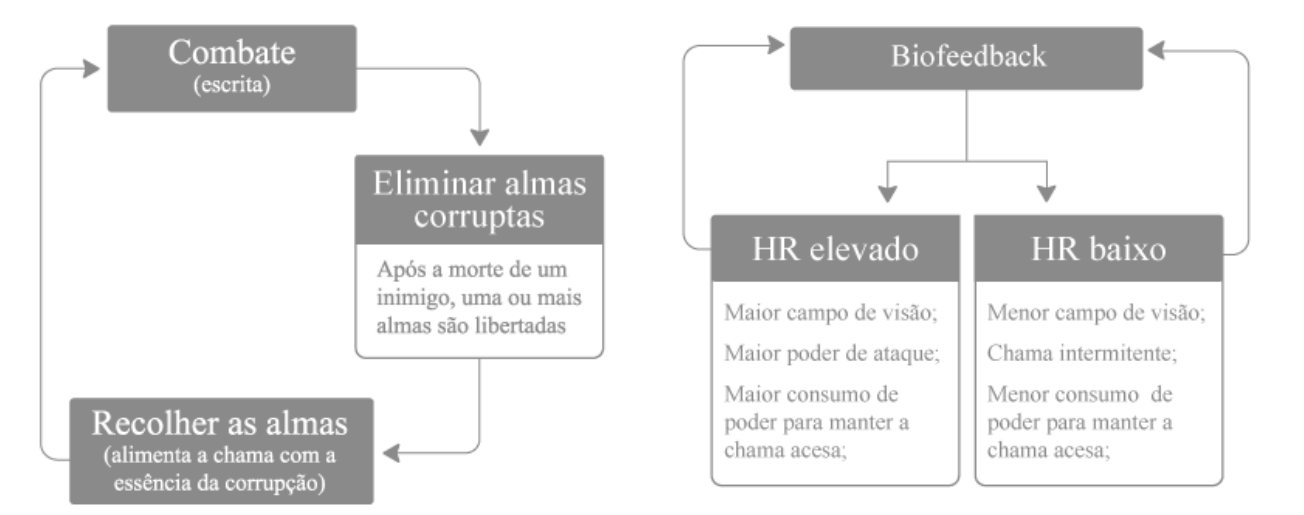
\includegraphics[width=17cm]{Figuras/diagrama-filipa-loop.png}
    \caption*{Fonte: \cite{filipa2019emovere}}
    \label{fig:diagrama_biofeedback}
\end{figure}

Os trabalhos apresentados conseguem cobrir com clareza os aspectos técnicos da implementação, através de métodos e materiais conhecidos e replicáveis. Buscamos aplicar alguns destes conhecimentos neste projeto, sendo eles a game engine Unity e o loop de biofeedback entre jogador e jogo.

Nota-se que grande parte dos recursos e conceitos extraídos e analisados nos trabalhos acima não serão utilizados neste trabalho. Isso se deve ao fato de que, na metodologia que será abordada aqui, não será utilizada detecção em tempo real. Isso está melhor descrito em \ref{metodologia}.

Além destes conteúdos, utilizamos metodologias para leituras de arquivos com dados de sinais neurais e sinais fisiológicos, técnicas de game development e integração de sistemas para agregar o jogo a um sistema de interpretação. Esses processos também estão detalhados em \ref{metodologia} 

Serão focados neste trabalho tentativas para expandir o que foi abordado nos dois projetos mencionados: enquanto ambos trabalham apenas com sinais fisiológicos, serão trabalhados entradas de sinais neurais reconhecidos.